% -------------------------------------------------------------------------------------------------
%      MDSG Latex Framework
%      ============================================================================================
%      File:                  main.tex
%      Author(s):             Michael Duerr
%      Version:               1
%      Creation Date:         30. Mai 2010
%      Creation Date:         30. Mai 2010
%
%      Notes:                 - This represents the document root of this template
%                             - Binding correction is 12mm. In case you change this value, you
%                               may also need to adapt the value of \bcorlength in mdsg.sty
%                             - Switch `babel' package options `english' and `ngerman' in case
%                               your thesis is in English
%                             - if you prefer to use utf8 encoding, uncomment the corresponding
%                               line `\usepackage[utf8]{inputenc}' and comment the line
%                               `\usepackage[latin1]{inputenc}'. To compile this example you also
%                               need to include the corresponding introduction example file i.e.
%                               `introduction-UTF8.tex' or `introduction-ISO8859-1.tex'
% -------------------------------------------------------------------------------------------------
%
\documentclass[enabledeprecatedfontcommands,bibliography=totoc,listof=totoc,index=totoc,twoside=true,BCOR=12mm,DIV=12]{scrbook}
%\KOMAoptions{draft=true}                         % uncomment if you want to visualise overful hbox
%\KOMAoptions{chapterprefix=true}                 % uncomment if you like "Chapter" in front of
                                                  % chapter number
%\KOMAoptions{appendixprefix=true}                % uncomment if you like "Appendix" in front of
                                                  % appendix number
%\KOMAoptions{...}                                % feel free to add additional KOMA options
%
% =================================================================================================
% set encoding
% -------------------------------------------------------------------------------------------------
%
\usepackage[utf8]{inputenc}                       % uncomment if you prefer utf8 encoding
%\usepackage[latin1]{inputenc}                    % uncomment if you prefer latin1 encoding
%
% =================================================================================================
% load mdsg style
% -------------------------------------------------------------------------------------------------
%
%\usepackage[diplom]{mdsg}                        % uncomment the corresponding option
%\usepackage[fopra]{mdsg}
\usepackage[bachelor]{mdsg}
%\usepackage[master]{mdsg}
%
% =================================================================================================
% initialize macros
% -------------------------------------------------------------------------------------------------
%
\lmutitle{Titel der Arbeit}                       % title: you can force a new line by
%\lmutitle{Titel \\ der \\ Arbeit}                % inserting `\\'. However, this will cause
                                                  % a hyperref warning!
\lmustudentone{Tim Hesse}                         % first author's name
%\lmustudenttwo{Max2 Mustermann2}                 % second author's name
%\lmustudentthree{Max3 Mustermann3}               % third author's name
%\lmustudentfour{Max4 Mustermann4}                % fourth author's name

\lmuprofone{Prof. Dr. Claudia Linnhoff-Popien}    % first supervisor's name
%\lmuproftwo{Prof. Dr. Max Mustermann}             % second supervisor's name
                                                  % (uncomment if not needed)
%\lmuprofthree{Prof. Dr. Max2 Mustermann2}         % third supervisor's name
                                                  % (uncomment if not needed)
\lmuadvisorone{Thomas Gabor}                    % first advisor's name
\lmuadvisortwo{Thommy Phan}                    % second advisor's name
                                                  % (uncomment if not needed)
%\lmuadvisorthree{Betreuer Name3}                  % third advisor's name
                                                  % (uncomment if not needed)
\lmudraftdate{\today}                             % only for versioning during work!
                                                  % (uncomment for final version!)
\lmudeadline{15. Juli 2021}                      % deadline (day of submission)
%
% =================================================================================================
% package selection (add additional packages if needed)
% -------------------------------------------------------------------------------------------------
%
%\usepackage{layout}                              % see documentation of this package
\usepackage{cmap}                                 % to produce searchable PDF
\usepackage[T1]{fontenc}                          % split german words with umlaut
\usepackage{lmodern}
\usepackage[english,ngerman]{babel}               % for german toc, ...
\usepackage{bibgerm}                              % for german bibliography index
\usepackage{tabularx}                             % more flexible table environment
\usepackage{booktabs}                             % high quality tables
\usepackage{rotating}                             % for generation of landscape tables
\usepackage{multirow}                             % for multirow cells inside tables
\usepackage{amssymb,amsmath}                      % powerful math package
\usepackage{hyperref}                             % for hyperlinks
\lmuhypersetup                                    % write some pdf properties
\usepackage{flafter}                              % force floats to appear after their reference
\usepackage{subfig}                               % to allow for side by side graphics (subfloats)
\usepackage{pdflscape}                            % enable rotation of landscape pages
\usepackage{hyphenat}                             % proper hyphenation for bla_bla to bla_-bla
\usepackage[all]{hypcap}                          % correct captions
\usepackage{url}                                  % nicer url style
\usepackage{enumitem}                             % for tight lists
%\usepackage{...}                                 % add additional packages here

\setcounter{tocdepth}{3}                          % sectioning depth in toc
\setcounter{secnumdepth}{3}                       % sectioning depth in text

\graphicspath{{./pictures/}}                      % put all graphics here
% -------------------------------------------------------------------------------------------------
%      MDSG Latex Framework
%      ============================================================================================
%      File:                  hyphenation.tex
%      Author(s):             Michael Duerr
%      Version:               1
%      Creation Date:         30. Mai 2010
%      Creation Date:         30. Mai 2010
%
%      Notes:                 - Instruction \hypenation cannot handle special characters like umlaute
%                               as well as  "a and \"a. Split such words in your text.
%
% -------------------------------------------------------------------------------------------------
%
\hyphenation{Ba-che-lor-ar-}
%\hyphenation{...}                           % further hyphenation examples
                               % this file holds words latex cannot split
%
% =================================================================================================
% start of document
% -------------------------------------------------------------------------------------------------
%
\begin{document}
    \setlist{noitemsep}                           % for tight lists
    \lmufront                                     % title pages
    \newpage
    \cleardoublepage
    \lmuaffirmation                               % affirmation (work is my own work)
    \newpage
    \cleardoubleemptypage
    \thispagestyle{empty}
%    % -------------------------------------------------------------------------------------------------
%      MDSG Latex Framework
%      ============================================================================================
%      File:                  abstract.tex
%      Author(s):             Michael Duerr
%      Version:               1
%      Creation Date:         30. Mai 2010
%      Creation Date:         30. Mai 2010
%
%      Notes:                 - Place your abstract here
% -------------------------------------------------------------------------------------------------
%
\vspace*{2cm}

\begin{center}
    \textbf{Abstract}
\end{center}

\vspace*{1cm}

\noindent In recent years reinforcement learning(RL) showed substantial improvement in perfect information games such
as Chess or Go compared to traditional heuristic based approaches.\\
The aim of this work was to explore the capabilities of RL in games that do not feature perfect information.
As a case study we chose the bavarian card game Schafkopf, which is a 4 player trick game that features contract
bidding, including solo and team play.
We employed the well established \textbf{Proximal Policy Optimisation} algorithm to train two agents, that use two
different approaches generating training data, to play against our own baselines(Random, Greedy, Heuristic) in a custom
\textbf{multi-agent} environment using \textbf{Python}.
By fixing the contract bidding, we were able to accurately evaluate the playing strength of our agents.
We were able to beat the Random baseline convincingly, while failing to beat the two stronger rule based players.
                       % abstract
    \thispagestyle{empty}
    \frontmatter                                  % start roman numbering
    \tableofcontents                              % toc
    \mainmatter                                   % start alpha numbering
%
% =================================================================================================
% place your document text here (take care of encoding)
% -------------------------------------------------------------------------------------------------
%
    %\input{text/introduction-UTF8}
    %% -------------------------------------------------------------------------------------------------
%      MDSG Latex Framework
%      ============================================================================================
%      File:                  introduction-[UTF8,ISO8859-1].tex
%      Author(s):             Michael Duerr
%      Version:               1
%      Creation Date:         30. Mai 2010
%      Creation Date:         30. Mai 2010
%
%      Notes:                 - Example chapter
% -------------------------------------------------------------------------------------------------
%
\chapter{Einleitung}\label{sec:Introduction}
Dies ist der \LaTeX\ Rahmen zur Bearbeitung von Bachelor-, Master-, Projekt- und Diplomarbeiten.
Alle relevanten Dateien befinden sich im Verzeichnis \verb|text|.
\section{Unterverzeichnisse und Dateien}
Das Verzeichnis \verb|text| beinhaltet weitere Unterverzeichnisse und Dateien, die den Rahmen charakterisieren.
\subsection{\textbf{main.tex}}\label{subsec:main}
Diese Datei stellt die zentrale Konfigurationsdatei f�r den Rahmen dar. Unter anderem m�ssen hier Informationen
�ber die Aufgabensteller, Betreuer, die Art der Arbeit sowie deren Title eingestellt werden.
Hier k�nnen auch weitere Pakete eingebunden werden. Die Datei ist dokumentiert und sollte selbsterkl�rend
sein.
\subsection{\textbf{hyphenation.tex}}
Manche W�rter werden von \LaTeX\ nicht (ordentlich) getrennt. Diese k�nnen in dieser Datei mit deren
Trennungsstellen hinzugef�gt werden.
\subsection{\textbf{Makefile}}
Um das Dokument zu erstellen muss man den Aufruf \verb|make all| t�tigen. Dabei werden einige tempor�re
Dateien erstellt sowie die Datei \verb|main.pdf| die das entsprechende Dokument enth�lt. Mir dem
Aufruf \verb|make clean| werden alle tempor�ren Dateien sowie die Datei \verb|main.pdf| gel�scht.
sie k�nnen die Datei \verb|Makefile| ihren Anforderungen entsprechend erweitern.
\subsection{\textbf{text}}
Es bietet sich an f�r verschiedene Kapitel eigene Quelldateien zu pflegen. Diese sollten sie alle im
Ordner \verb|text| ablegen. Wie ein Kapitel eingebunden wird, kann man aus dem Beispiel in der
Datei \verb|main.tex| ablesen. Das Verzeichnis \textbf{text} beinhaltet zudem die Datei
\verb|abstract.tex|. In diese Datei soll eine kurze Zusammenfassung (ca. eine halbe Seite)
der Arbeit eingetragen werden. Die Datei \verb|appendix.tex| kann verwendet werden um einen
Anhang zu generieren.
\subsection{\textbf{pictures}}
Hier m�ssen sie alle Grafiken ablegen, die sie in ihrem Dokument einbinden wollen. Es sind nur die
Formate PDF, PNG und JPEG erlaubt (GIF ist m�glich, wird aber nicht empfohlen).
\subsection{\textbf{bibliography.bib}}
In diese Datei m�ssen alle Referenzen eingetragen werden,
die innerhalb ihrer Arbeit zitiert werden. Verwenden sie zur Verwaltung ihrer Referenzen einen
geeigneten Editor z.B. \textit{JabRef} (\url{http://jabref.sourceforge.net/}).
\subsection{\textbf{mdsg.sty}}
Hierbei handelt es sich um das Stylefile, das das Erscheinungsbild des Dokuments
lenkt. In dieser Datei sollten in der Regel keine Ver�nderungen notwendig sein.
\section{Beispiele}
Es gibt eine Unmenge an \LaTeX\ Tutorials und Dokumentationen, die guten Einstieg in das Arbeiten mit
\LaTeX\ erm�glichen. Im Folgenden werden aber ein paar undokumentierte Minimalbeispiele gegeben, die
den direkten Einstieg erm�glichen. Betrachten sie den Quelltext, um die Beispiele nachzuvollziehen.
\subsection{Zitate}
Wir zitieren hier eine Quelle von James Aspnes et al \cite{aspn07}, die in der  Datei\\
\verb|bibliography.bib|
steht.
\subsection{Listen}
Es gibt verschiedene M�glichkeiten Listen zu erstellen, z.B. ohne Nummerierung\dots
\begin{itemize}
   \item
      Das ist der erste Punkt,
      \begin{itemize}
         \item
            das der erste Unterpunkt,
         \item
            das der zweite Unterpunkt,
   \end{itemize}
   \item
      das der zweite, und
   \item
      das der dritte Punkt.
\end{itemize}
\dots oder mit Nummerierung\dots
\begin{enumerate}
   \item
      Das ist der erste Punkt,
      \begin{enumerate}
         \item
            das der erste Unterpunkt,
         \item
            das der zweite Unterpunkt,
      \end{enumerate}
   \item
      das der zweite, und
   \item
      das der dritte Punkt.
\end{enumerate}
\subsection{Referenz auf anderen Text}
Es ist auch m�glich auf andere Stellen im Text z.B. Kapitel \ref{subsec:main} zu verweisen.
\subsection{Hoch- und tiefgestellter Text}
Man kann Text tiefstellen indem man \verb|\textsubscript| verwendet, z.B. ergibt
\begin{verbatim}
text\textsubscript{tiefgestellt}
\end{verbatim}
den Text text\textsubscript{tiefgestellt}.
Das selbe funktioniert mit \verb|\textsuperscript| verwendet, z.B. ergibt
\begin{verbatim}
text\textsuperscript{hochgestellt}
\end{verbatim}
text\textsuperscript{hochgestellt}
\subsection{Tabellen}
Es gibt sch�ne M�glichkeiten Tabellen einzubinden wie z.B. Tabelle \ref{tab:CommonParameterSettings}.
\begin{center}
\begin{table}[htbp]
{\small
\begin{center}
\begin{tabular}[center]{lrlc}
\toprule
Parameter & Value & (Unit) & Available for Chord \\
\midrule
Query timeout & 10 & seconds & $\surd$ \\
Republish timeout & 300 & seconds & $\surd$ \\ % explain this value...
Stabilize timeout & 5 & seconds & $\surd$ \\
Fix fingers timeout & 30 & seconds & $\surd$ \\
Message timeout & 1 & second & $\surd$ \\
Connect timeout & 10 & seconds & $\surd$ \\
Ping superpeer timeout & 5 & seconds & $\times$ \\
Cost-Optimality estimation timeout & 20 & seconds & $\times$ \\
Significance for change in number of superpeers & 10 & percent & $\times$ \\
Significance for change in estimations  & 10 & percent & $\times$ \\
Number of permanent superpeers & 32 & nodes & $\times$ \\
Mean number of peers & 1000 & nodes & $\surd$ \\
Mean number of lookups per hour & 60 & queries & $\surd$ \\
Mean number of shared InfoProfiles per node & 20 & & $\surd$ \\
Identifier space & 16 & bits & $\surd$ \\
Direct insertion acknowledgment & true & bool & $\times$ \\
Direct query responses & true & bool & $\times$ \\
Force query resolution & true & bool & $\surd$  \\
\bottomrule
\end{tabular}
\end{center}
} % end of tiny
\caption[Simulation parameter settings]{Common simulation parameter settings.\label{tab:CommonParameterSettings}}
\end{table}
\end{center}

\subsection{Bilder}
Man kann sehr einfach Bilder einbinden so wie z.B. in Abbildung \ref{fig:pic0}.
\begin{figure}[hpbt]
  \centering
  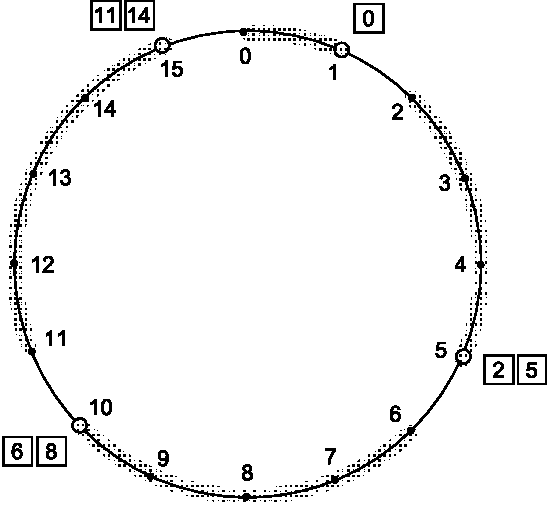
\includegraphics[width=0.4\textwidth]{pictures/pic0}\\
  \caption[Example of a $4$-bit Chord identifier circle]{Example of a $4$-bit Chord identifier circle.
  The responsibility ranges for each peer are accentuated in light gray}\label{fig:pic0}
\end{figure}
Es lassen sich auch mehrere Bilder nebeneinander platzieren wie z.B. in Abbildung
\ref{fig:multipic} zu sehen ist.
\begin{figure}[hpbt]
 \centering
  %%----start of first subfigure----
  \subfloat[FIFO size limited to 20 entries]{
   \label{fig:multipic:a} %% label for first subfigure
   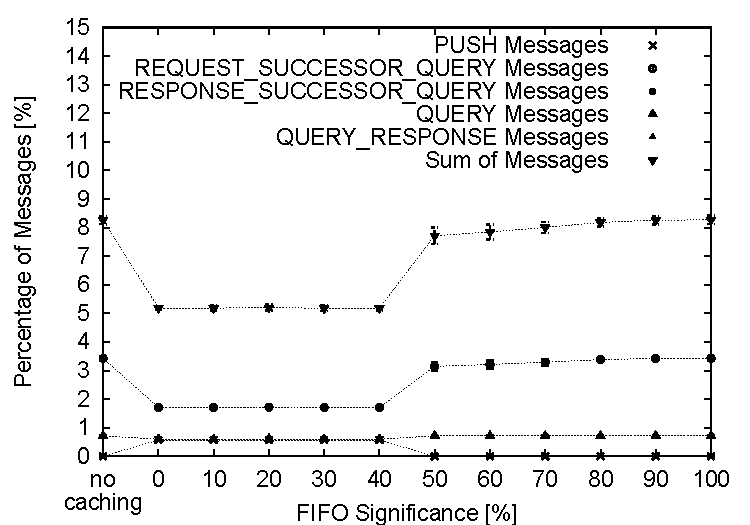
\includegraphics[width=0.48\linewidth]{pic1}}
  \hspace{0.01\textwidth}
  %%----start of second subfigure----
  \subfloat[FIFO size limited to 30 entries]{
   \label{fig:multipic:b} %% label for second subfigure
   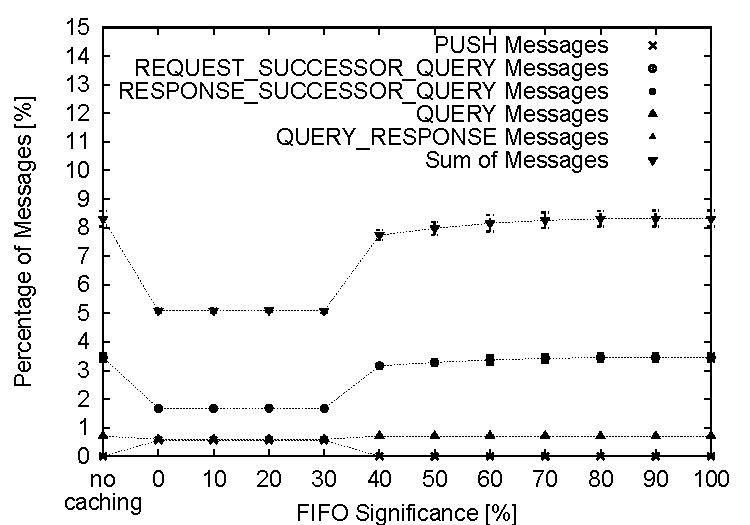
\includegraphics[width=0.48\linewidth]{pic2}}\\[0pt] % horizontal break
  %%----start of third subfigure----
  \subfloat[FIFO size limited to 40 entries]{
   \label{fig:multipic:c} %% label for third subfigure
   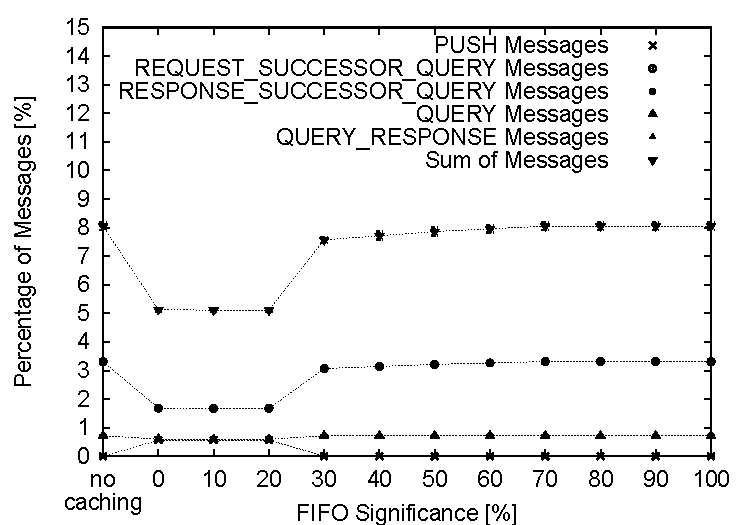
\includegraphics[width=0.48\linewidth]{pic3}}
  \hspace{0.01\textwidth}
  %%----start of fourth subfigure----
  \subfloat[FIFO size limited to 50 entries]{
   \label{fig:multipic:d} %% label for fourth subfigure
   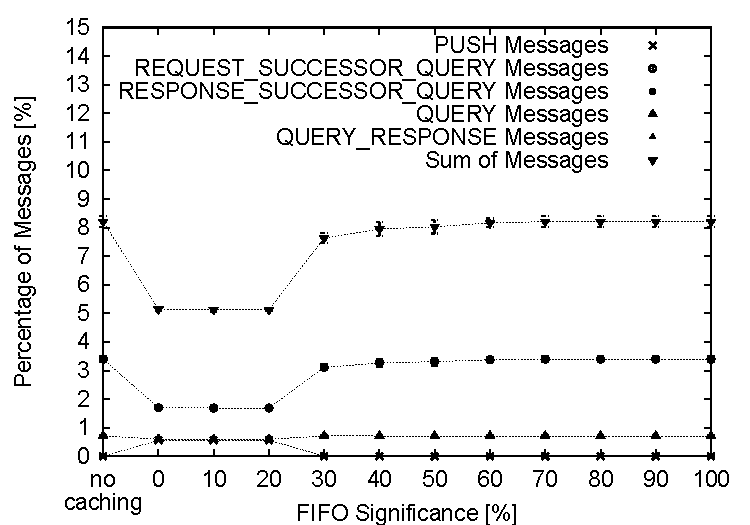
\includegraphics[width=0.48\linewidth]{pic4}}
 \caption[Observed message fractions and 95\% confidence intervals for Chord]{Observed message fractions and 95\% confidence intervals for Chord without the influence of churn. The FIFO capacity varies from 20 (\ref{fig:multipic:a}) -- 50 (\ref{fig:multipic:d}) entries (decadic steps).}
 \label{fig:multipic} %% label for entire figure
\end{figure}

\subsection{Programm Code}
Eine elegante M�glichkeit, Programmtext einzubinden, l�sst sich mit dem listings-Paket erreichen.
Das \verb|HelloWorld| Programm aus Listing \ref{lst:hw} hat in Zeile \ref{line:hw3} �brigens einen Programmierfehler.
\begin{lstlisting}[float=htp,caption=Hello World,label=lst:hw,language=Java, numbers=left, numberstyle=\tiny, stepnumber=2, numbersep=8pt, escapeinside={//@}{@//},backgroundcolor=\color{yellow},xleftmargin=3ex,xrightmargin=1ex]
public class HelloWorld {
    public static void main(String[] args) {
        Syste.out.println("Hello, World"); //@\label{line:hw3}@//
    }
}
\end{lstlisting}

\subsection{Fu�noten}
Wenn man auf Google \footnote{\url{http://www.google.com}} verweisen will, bietet sich statt einer gesonderten
Referenz auch einfach eine Fu�note an.
\subsection{Formeln}
Man kann mit \LaTeX\ sehr sch�n Formeln erzeugen:
$$L_{P}(k) = R^{orig}_{P}(k) + \sum_{i=0}^n 2*R^{i}_{P}(k)$$

    % further chapters
    \chapter{Rules of Schafkopf}
Schafkopf is a traditional four player trump card game that is played in the south of Germany.
The game is widely popular for being easy to learn but allowing for deep strategies.
Often it is played for small money stakes.
A game of Schafkopf normally consists of multiple rounds of four hands, where the intial dealer position rotates
clockwise around the table.
In Order to play a hand players will bid between themselves for a game contract, creating either two teams of two or
two teams of one and three, and then play 8 tricks with differing rules sets that depend on the winning bid.


\section{Cards}\label{sec:cards}
The Game of Schafkopf uses a 32 card bavarian deck, containing 4 suits with 8 ranks each.
Since the bavarian deck is comparable with a 52 french deck, where all ranks 2-6 are excluded, we also included the
corresponding English names for each suit and rank in the following tables.
The following tables is ordered descendingly by strength.
\begin{table}[]
    \begin{tabular}{lll}
        Suit     & Short Hand & Corresponding French Suit \\
        Eichel   & E          & Clubs                     \\
        Gras     & G          & Spades                    \\
        Herz     & H          & Hearts                    \\
        Schellen & S          & Diamonds
    \end{tabular}\label{tab:table2}
\end{table}
Regardless of the contract each rank has a corresponding point value ranging from 11 to 0 points in discrete steps.
The total value of all 32 cards is therefore 120.
\begin{table}[]
    \begin{tabular}{llll}
        Rank  & Point Value & Short Hand & Corresponding French Rank \\
        Ass   & 11          & A          & Ace                       \\
        Zehn  & 10          & T          & Ten                       \\
        König & 4           & K          & King                      \\
        Ober  & 3           & O          & Queen                     \\
        Unter & 2           & U          & Jack                      \\
        9     & 0           & 9          & Nine                      \\
        8     & 0           & 8          & Eight                     \\
        7     & 0           & 7          & Seven
    \end{tabular}\label{tab:table}
\end{table}
In order to refer to cards in the future we also included a short hand way of expressing suit and rank.
For example the Ten of Herz is TH and the Ober of Gras is OG.


\section{Goal and Rules}

\subsection{Goal}
The goal is to score points by taking tricks, of which there are eight.
If a team after all cards are played has 61 points (60 for the opposition) the game is won.
The rulesset for Schafkopf depends on the contract that is being played, there are however a certain rules that
always apply.

\subsection{Trumps}
Schafkopf has a set of cards that are considered trump.
This set of cards is determined by the contract that is played.
Each set has an order of strenght that always follows the order of Ober > Unter > Color.
The suits themselves have also an order of Eichel > Gras > Herz > Schellen.
As an example the order of trumps for the most common contract Team, where all Ober, all Unter and all Herz are trump:
(OE,OG,OH,OS,UE,UG,UH,US,AH,TH,KH,9H,8H,7H)

\subsection{Trick}
There are two kinds of tricks, trump and suit.
The first card of each trick,it can either be of trump or a normal suit, determines which kind is present.
In both cases players behind must play a card of that suit/trump.
If they do not possess one of that kind they may play any other card, even trump if the first card played is a suit.
\newline
A suit trick can be won either by having the highest card suit on the table or by having the highest trump on the table.
Trump tricks can however only be won by playing the highest trump.
There is no obligation to win a trick if you can do so.
Other restrictions and obligations on which cards can be played will be introduced in the Team contract section,
but the above rules are sufficient in most cases.
\section{Game Phases}
At the beginning of each player is seated at the table, and a player is randomly chosen to deal.
The initial seating relative to one another should not be changed, since the dealer position rotates after each hand
clockwise, thus
skewing the fairness.
\newline
Every hand of Schafkopf can be broken down in four distinct phases:
\begin{enumerate}
    \item Setup Phase
    \item Bidding Phase
    \item Trick Phase
    \item Scoring Phase
\end{enumerate}
To avoid complexity we excluded the doubling stage (players can choose to double the final hand reward after they
receive the first half of their hand), and the Contra stage (opposition players may double the stakes after the first card is played)
\subsection{Setup Phase}
At the beginning of a hand the player in the dealer position shuffles the cards and deals each player a hand of eight
cards.
This player is called the Dealer, and the player to his immediate left has the Lead.
\subsection{Bidding Phase}
The player with the lead starts the bidding phase and can either announce Pass or Play, then the next player clockwise announces his bid.
This continues until all players announced their intentions.
If a any previous player anounced Play, players may only also announce Play if they intend to chose a Solo Mode.
If every player passes, the hand ends and the current dealer reshuffels the cards and returns to
the Setup Phase.
If only one player announced Play, he announces his chosen contract and the Trick Phase begins.
If more than one player announced Play, the players with the highest bid wins the bid.
The order goes TEAM < WENZ < SOLO
\subsection{Trick Phase}
The player with the Lead plays his first card and the play continues in clockwise order until everybody played one
card.
The winner of the of the current trick collects all cards and becomes the new Lead.
After all eight tricks have been played the game moves into the scoring phase.
\subsection{Scoring Phase}
Each team counts their combined points, and a winner is determined.
The team that won the bid requires 61 points, whilst the opposition team only requires 60 points.
The rewards can now be calculated using a prearranged structure.
The base value of a game depends on the contract
that is being played,where SOLO modes are rewarded more due to their higher risk.
\newline
There are also specials rewards a team can earn:
\begin{description}
    \item[Schneider] The bid winners can claims Schneider when the opposition has not scored 30 points and vice versa
    if the bid winners have not scored 31 points.
    \item[Schwarz] A winning team can claim Schwarz if the other team have not won a single trick. A trick with 0
    points still counts as trick win.
    \item[Laufende] Laufende is a row of the highest trumps held by a party without interruption.
    In the TEAM game and COLOR Solo, payment is made from three Laufende (at least OE,OG,OH) and in the WENZ,
    payment is made from two Laufende (at leas UE,UG). Laufende can range from 2 up to 14 depening which contract is
    played.
\end{description}
The formula to calculate the final hand reward is always:
\begin{equation*}
    Hand Reward = Base Reward + Schneider + Schwarz + Laufende
\end{equation*}
Losers pay the winner the Hand rewards paid out always sum up to zero.
In TEAM game the losers get the negative hand reward, and the winners receive the positive hand reward.
In SOLO the bid winner receives three time the reward and each player receives a single hand reward.
The structure used in this paper can be found in the following table.
The hand is now finished, and the dealer role rotates clockwise.
\begin{table}[]
\begin{tabular}{ll}
Name     & Base Reward \\
Specials & 10          \\
Team     & 20          \\
Solo     & 50    
\end{tabular}\label{tab:table3}
\end{table}
\section{Contracts}
Schafkopf has a lot of differing contracts,these often allow for more Solo contracts or avoid aborting the hand.
All contracts follow the same trick rules we defined ealier, and only differ in the way the players are divided in
teams,what cards are Trump and the order of card ranks.
For this implementation we considered only the three classic contracts:
\begin{itemize}
    \item Team Mode
    \item Wenz
    \item Color Solo
\end{itemize}
Team mode is a two vs two variant and most, whilst WENZ and COLOR SOLO both pit the bid winner against the other three.

\subsection{Team}
In the Team game there are 14 Trumps, four Ober, four Unter and all Herz.
\newline
The bid winner calls a color ace that she does not hold herself, but she must hold at least one card of that color
that is not trump.
The player that holds the ace, being called the partner, will be allied for with the bid winner, whilst the remaining
players form the opposition team.
\newline
\begin{figure}
    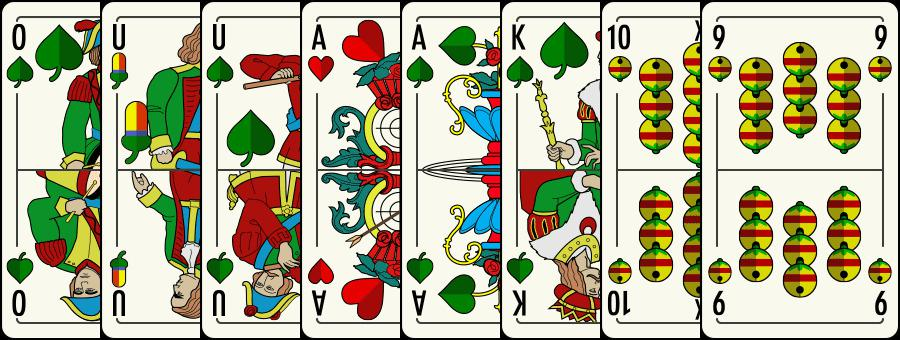
\includegraphics[scale=0.5]{partnerBiddingExample}\label{fig:figure}
    \caption{The player can only search for AS, since he holds the AG himself and has no Eichel himself}
\end{figure}
At the beginning of the hand only the partner knows the full team compositions, but in normal play this becomes
apparent fairly soon, can sometimes however last until the last trick.
If a trick starts with the searched color, the Partner has to play the ace.
This process is called Searching and reveals the team composition.
The partner may play the Ace at the beginning of a trick himself if he has the lead.
If no one searches the ace may only be played in the last trick.
If the partner has a four cards of the searched suit,including the ace, he may run away by playing a different card of
that suit, if and only if he has the lead.
Once runaway he may play the ace at any point.
This is due to the fact that if he holds 4 cards of the suit, the bid winner one, there is only one remaining cards
with the opposition.
This would guarantee a lost trick if the opposition searches and holds trump.

\subsection{Solos}
The Solos require a much stronger hand in general in order to win.

\subsubsection{Suit Solo}
The bid winner calls which color is trump.
As with the Team game there are 14 Trumps, four Ober, four Unter and six cards of the chosen color.
The team composition is obvious after the bid winner announces his game.

\subsubsection{Wenz Solo}
In the Wenz Solo the only trumps are the four Unter.
The Ober are now considered color and slot in after the King in terms of card ranking.


\section{Basic Strategy}
Schafkopf is a game with a lot of subtle and deep strategies that can take a many hands to master, yet most beginners
are given a set of base rules to follow.
Most of these rules are role dependent and will be outlined shortly below.

\subsection{Search and runaway when possible}
Players should always search when they have the chance.
Since at least two of the six searched suit cards are between the bid winner and her partner and one is with herself
the chance is high that her partner holds no cards of that suit and can trump.
The more cards of the suit he holds himself, the more likely it is that his partner is free.
Another benefit of searching is to gain information about the team composition, since the opposition knows the least
about it.\\
Due to the natural imbalance of trumps between the two teams, the oppostion will most likely score fewer tricks and
thus gains from knowing who their partner is.
This way they can use their trumps and high scoring cards more efficiently.
\newline
The searched partner in a team should always run away when he holds four suit cards in order to reduce the points lost
to the opposition.
This way he saves the 11 points of the ace for a later trick.
A rare exeption to the rule is when the searched player holds 5 cards and the bid winner the last.
In this case running away is pointless since the opposition has no means of searching in the first place.
\newline
Although this rule only applies to players that have the lead, it can still be useful in other situations.
For example when players have the chance to take the lead by winning a trick only as a means to search or run away in
the following trick.
This can sometimes mean taking away a trick of the partner or winning a low scoring trick.

\subsection{Bidder plays Trump,oppositon plays color}
This rule refers to the decision when a player has the lead, and applies to both Solo and team games.
Since the bid winner announced the game he should have more trumps than the other players and thus also fewer colors.
By playing trump when he has the lead, he can drain the opposition's trumps.
After the opposition no longer holds trump, consecutive colors such as [A,T,K] gain in strength as they cannot be
trumped anymore.
If the player had played color from the beginning, the trick could have been lost.\\
In team mode this rule also applies to the searched player and often serves as a way of signaling team membership,
since playing trump and being on the opposition in general is counterproductive.
\newline
The reverse logic applies to the opposition's strategy, as they have fewer trumps they should use the lead as an
opportunity to play color to see if they can score this way as it is unlikely to make many tricks
with trump.
If a player has aces he should play them early, before the bid winner can rid himself of that color, or play a low
color in the hope that his partner holds the ace or has trump left in case he does not hold the color himself.
\newline
In team games this strategy also servers as way of signalling team membership, especially if the lead in the first
trick opens with a suit that is not the searched ace.
By not playing trump and not searching the player signals he is part of the opposition and can not search.
His partner in turn should thus try to gain the lead in order to search before the other team drains all their trumps.

\subsection{}


%
% =================================================================================================
% place your appendix here
% -------------------------------------------------------------------------------------------------
%
    \appendix
    % -------------------------------------------------------------------------------------------------
%      MDSG Latex Framework
%      ============================================================================================
%      File:                  appendix.tex
%      Author(s):             Michael Duerr
%      Version:               1
%      Creation Date:         30. Mai 2010
%      Creation Date:         30. Mai 2010
%
%      Notes:                 - Place your appendix here
%                             - Use the same commands (`chapter', `section', ...) as in main text
% -------------------------------------------------------------------------------------------------
%
\chapter{Beispiel Anhang}
\small{
\begin{verbatim}
/*
* This code serves the initialization of an auxiliary probability array.
* The array holds at each position a pre-calculated probability for the index
* of that position. The probability reflects the Zipf-distribution for the
* corresponding indexes
*/
Set zipfExponent to 1.4
Set sum to 0
Set maxInteger to 65535
FOR i = 0 to maxInteger
probArray[i] = 1/pow(i + 1, zipfExponent)
Set sum = sum + probArray[i]
END FOR
FOR i = 0 to maxInteger
Set probArray[i] = probArray[i]/sum
END FOR
FOR i = 1 to maxInteger
Set probArray[i] = probArray[i] + probArray[i] = probArray[i-1]
END FOR

/*
* This code gets called in case a Zipf-distributed number is required. It
* iterates over the probability array until the chosen random number v
* is less than the value stored at the current array position i. The value of
* the array position will be returned as the calculated Zipf-distributed
* number
*/
Set v to a random number between 0 and 1
FOR i = 0 to maxInteger
IF v < probArray[i] THEN
RETURN i
END IF
END FOR
RETURN 0

\end{verbatim}
}

    % further appendix
%
% =================================================================================================
% comment \listoffigures and/or \listoftables if not wanted
% -------------------------------------------------------------------------------------------------
%
    \backmatter
    \listoffigures                                % list of figures (uncomment if wanted)
    \listoftables                                 % list of tables (uncomment if wanted)
    \lstlistoflistings                            % list of listings (uncomment if wanted)
%
% =================================================================================================
% place your bibliography here
% -------------------------------------------------------------------------------------------------
%
    \begin{spacing}{0.9}                          % save some space
       \bibliographystyle{geralpha}               % for german thesis
       %\bibliographystyle{alpha}                 % for english thesis
       \bibliography{bibliography}                % the location of bib file
    \end{spacing}
\end{document}
%
% =================================================================================================
% end of document
% -------------------------------------------------------------------------------------------------
%